% ============================================================
%  L01_mini5.tex  --  Fintech Foundations and Overview
%  5-Slide Teaser Arc: WHY > WHAT > HOW > WHERE > SO WHAT
%  Self-contained (no \input{} commands, no \includegraphics)
%  Compile: pdflatex L01_mini5.tex  (twice for overlays)
% ============================================================

\documentclass[aspectratio=169, 11pt]{beamer}
\usetheme{Madrid}
\usecolortheme{whale}
\usepackage{tikz,pgfplots,booktabs,multicol,amsmath}
\usetikzlibrary{arrows.meta,positioning,shapes.geometric,calc,decorations.pathmorphing}
\pgfplotsset{compat=1.18}

% ---- Colour palette ----------------------------------------
\definecolor{mlpurple}{HTML}{9467BD}
\definecolor{mlblue}{HTML}{1F77B4}
\definecolor{mlred}{HTML}{D62728}
\definecolor{mlorange}{HTML}{FF7F0E}
\definecolor{mlgreen}{HTML}{2CA02C}
\definecolor{mlgray}{HTML}{7F7F7F}
\definecolor{mlteal}{HTML}{0D7377}
\definecolor{mlcyan}{HTML}{14BDEB}

% ---- Beamer theme colours ----------------------------------
\setbeamercolor{structure}{fg=mlteal}
\setbeamercolor{palette primary}{bg=mlteal,fg=white}
\setbeamercolor{palette secondary}{bg=mlteal!80,fg=white}
\setbeamercolor{palette tertiary}{bg=mlteal!60,fg=white}
\setbeamercolor{frametitle}{bg=mlteal!10,fg=mlteal}
\setbeamercolor{title}{fg=white}
\setbeamercolor{subtitle}{fg=mlcyan!80}
\setbeamercolor{block title}{bg=mlteal,fg=white}
\setbeamercolor{block body}{bg=mlteal!8,fg=black}
\setbeamercolor{block title alerted}{bg=mlred!80,fg=white}
\setbeamercolor{block body alerted}{bg=mlred!8,fg=black}

% ---- Bottom-note command -----------------------------------
\newcommand{\bottomnote}[1]{%
  \vfill
  \begin{beamercolorbox}[wd=\textwidth,ht=2ex,dp=1ex]{palette primary}%
    \tiny\hspace{1em}#1%
  \end{beamercolorbox}}

% ---- Metadata ----------------------------------------------
\title{Fintech Foundations and Overview}
\subtitle{5-Slide Teaser}
\author{Joerg Osterrieder}
\institute{University of Zurich}
\date{Spring 2026}
\setbeamertemplate{navigation symbols}{}

% ============================================================
\begin{document}
% ============================================================

% -----------------------------------------------------------
%  TITLE FRAME (not counted in the 5)
% -----------------------------------------------------------
\begin{frame}
  \titlepage
  \bottomnote{Financial Technology (FinTech) -- MSc Course | University of Zurich | Spring 2026}
\end{frame}

% ===========================================================
%  SLIDE 1 of 5  --  WHY
%  Visual: TikZ comic -- banker vs. fintech founder
% ===========================================================
\begin{frame}{Why Now? The Disruption Moment}

\begin{center}
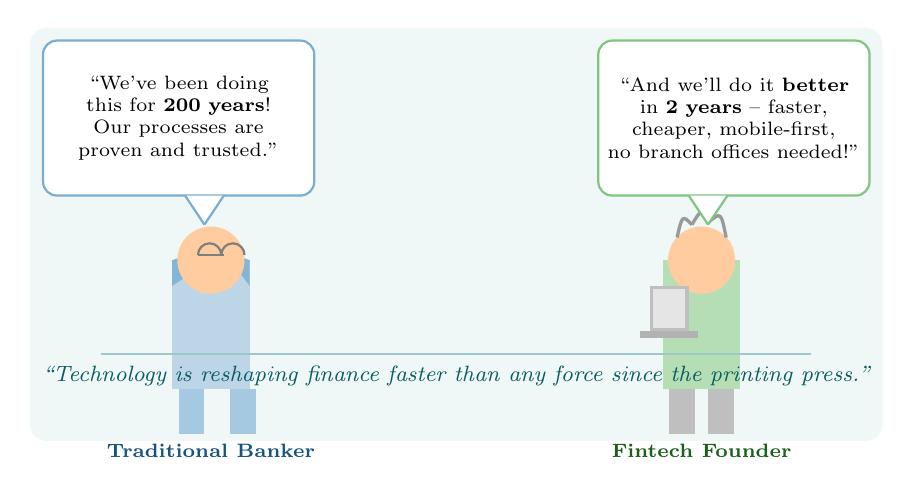
\begin{tikzpicture}[scale=0.82, every node/.style={font=\small}]

  % ---- Background strip ----
  \fill[mlteal!6, rounded corners=6pt]
    (-6.6,-2.6) rectangle (6.6,3.8);

  % ---- BANKER (left) ----
  % Body
  \fill[mlblue!30] (-4.4,-1.8) rectangle (-3.2,0.2);
  % Suit lapels
  \fill[mlblue!55] (-4.4,-0.2) -- (-3.8,0.2) -- (-3.5,0.2) -- (-3.2,-0.2) -- (-3.2,0.2) -- (-3.8,0.4) -- (-4.4,0.2) -- cycle;
  % Head
  \fill[mlorange!40] (-3.8,0.2) circle (0.52);
  % Glasses
  \draw[mlgray,thick] (-4.0,0.28) -- (-3.6,0.28);
  \draw[mlgray,thick] (-4.0,0.28) arc(180:0:0.18);
  \draw[mlgray,thick] (-3.64,0.28) arc(180:0:0.18);
  % Legs
  \fill[mlblue!40] (-4.3,-1.8) rectangle (-3.9,-2.5);
  \fill[mlblue!40] (-3.5,-1.8) rectangle (-3.1,-2.5);
  % Label
  \node[mlblue!70!black, font=\scriptsize\bfseries] at (-3.8,-2.75) {Traditional Banker};

  % ---- FINTECH FOUNDER (right) ----
  % Body (t-shirt)
  \fill[mlgreen!35] (3.2,-1.8) rectangle (4.4,0.2);
  % Head
  \fill[mlorange!40] (3.8,0.2) circle (0.52);
  % Hair (messy)
  \draw[mlgray!80, line width=1.2pt] (3.42,0.55) .. controls (3.5,0.9) .. (3.65,0.75);
  \draw[mlgray!80, line width=1.2pt] (3.65,0.75) .. controls (3.8,1.0) .. (3.9,0.78);
  \draw[mlgray!80, line width=1.2pt] (3.9,0.78) .. controls (4.1,0.95) .. (4.18,0.55);
  % Laptop in hand
  \fill[mlgray!50] (3.0,-0.9) rectangle (3.6,-0.2);
  \fill[mlgray!20] (3.05,-0.85) rectangle (3.55,-0.25);
  \fill[mlgray!60] (2.85,-0.9) rectangle (3.75,-1.0);
  % Legs
  \fill[mlgray!50] (3.3,-1.8) rectangle (3.7,-2.5);
  \fill[mlgray!50] (3.9,-1.8) rectangle (4.3,-2.5);
  % Label
  \node[mlgreen!60!black, font=\scriptsize\bfseries] at (3.8,-2.75) {Fintech Founder};

  % ---- BANKER speech bubble ----
  \fill[white, rounded corners=5pt]
    (-6.4,1.2) rectangle (-2.2,3.6);
  \draw[mlblue!60, rounded corners=5pt, line width=0.8pt]
    (-6.4,1.2) rectangle (-2.2,3.6);
  % Tail pointing to banker head
  \fill[white] (-4.2,1.2) -- (-3.9,0.75) -- (-3.6,1.2) -- cycle;
  \draw[mlblue!60, line width=0.8pt] (-4.2,1.2) -- (-3.9,0.75);
  \draw[mlblue!60, line width=0.8pt] (-3.9,0.75) -- (-3.6,1.2);
  \node[align=center, font=\scriptsize, text width=3.6cm] at (-4.3,2.4) {``We've been doing\\this for \textbf{200 years}!\\Our processes are\\proven and trusted.''};

  % ---- FOUNDER speech bubble ----
  \fill[white, rounded corners=5pt]
    (2.2,1.2) rectangle (6.4,3.6);
  \draw[mlgreen!60, rounded corners=5pt, line width=0.8pt]
    (2.2,1.2) rectangle (6.4,3.6);
  % Tail pointing to founder head
  \fill[white] (3.6,1.2) -- (3.9,0.75) -- (4.2,1.2) -- cycle;
  \draw[mlgreen!60, line width=0.8pt] (3.6,1.2) -- (3.9,0.75);
  \draw[mlgreen!60, line width=0.8pt] (3.9,0.75) -- (4.2,1.2);
  \node[align=center, font=\scriptsize, text width=3.6cm] at (4.3,2.4) {``And we'll do it \textbf{better}\\in \textbf{2 years} -- faster,\\cheaper, mobile-first,\\no branch offices needed!''};

  % ---- Core tension caption ----
  \node[mlteal!80!black, font=\footnotesize\itshape, align=center]
    at (0,-1.6) {``Technology is reshaping finance faster than any force since the printing press.''};
  \draw[mlteal!40, line width=0.6pt] (-5.5,-1.25) -- (5.5,-1.25);

\end{tikzpicture}
\end{center}

\bottomnote{Slide 1/5 -- WHY | Core tension: Is fintech replacing banks, or are banks becoming fintech?}
\end{frame}

% ===========================================================
%  SLIDE 2 of 5  --  WHAT
%  Visual: booktabs comparison table
% ===========================================================
\begin{frame}[shrink=8]{What Makes Fintech Different?}

\vspace{-0.2em}
\begin{columns}[T]
\begin{column}{0.52\textwidth}
  \begin{center}
  \scriptsize
  \setlength{\tabcolsep}{4pt}
  \renewcommand{\arraystretch}{1.18}
  \begin{tabular}{@{}lll@{}}
    \toprule
    \textbf{Dimension} & \textbf{Traditional Bank} & \textbf{Fintech} \\
    \midrule
    \textbf{Speed} & Days / weeks & Seconds / minutes \\
    \textbf{Cost} & Branch overhead & Near-zero marginal \\
    \textbf{Access} & Geography-limited & Smartphone = branch \\
    \textbf{Experience} & Form-heavy, opaque & Intuitive, real-time \\
    \textbf{Innovation} & Internal, slow cycles & Rapid iteration \\
    \textbf{Regulation} & Comprehensive & Evolving / patchy \\
    \bottomrule
  \end{tabular}
  \end{center}
  \vspace{0.2em}
  \begin{block}{Key Insight}
    \scriptsize Fintech reimagines \emph{how} financial services are delivered -- not whether they exist.
  \end{block}
\end{column}
\begin{column}{0.45\textwidth}
  \vspace{0.1em}
  \textcolor{mlteal}{\textbf{\small Seven Fintech Verticals}}
  \vspace{0.2em}
  \begin{itemize}\scriptsize
    \setlength{\itemsep}{2pt}
    \item[\textcolor{mlteal}{$\blacktriangleright$}] \textbf{Payments} -- mobile wallets, real-time
    \item[\textcolor{mlteal}{$\blacktriangleright$}] \textbf{Lending} -- P2P, BNPL, alt-scoring
    \item[\textcolor{mlteal}{$\blacktriangleright$}] \textbf{Insurtech} -- on-demand, parametric
    \item[\textcolor{mlteal}{$\blacktriangleright$}] \textbf{WealthTech} -- robo-advisors, micro-investing
    \item[\textcolor{mlteal}{$\blacktriangleright$}] \textbf{Capital Markets} -- tokenisation
    \item[\textcolor{mlteal}{$\blacktriangleright$}] \textbf{RegTech} -- compliance automation
    \item[\textcolor{mlteal}{$\blacktriangleright$}] \textbf{Banking Infra} -- neobanks, BaaS, APIs
  \end{itemize}
  \vspace{0.2em}
  \begin{alertblock}{\scriptsize Fintech Defined}
    \tiny Technology-enabled innovation creating new financial products, processes, or \emph{business models}.
  \end{alertblock}
\end{column}
\end{columns}

\bottomnote{Slide 2/5 -- WHAT | ``Fintech is not a product -- it is a force that reshapes how financial services are created, delivered, and consumed.''}
\end{frame}

% ===========================================================
%  SLIDE 3 of 5  --  HOW
%  Visual: TikZ architecture -- 4 collaboration models
% ===========================================================
\begin{frame}{How Do Banks and Fintechs Work Together?}

\begin{center}
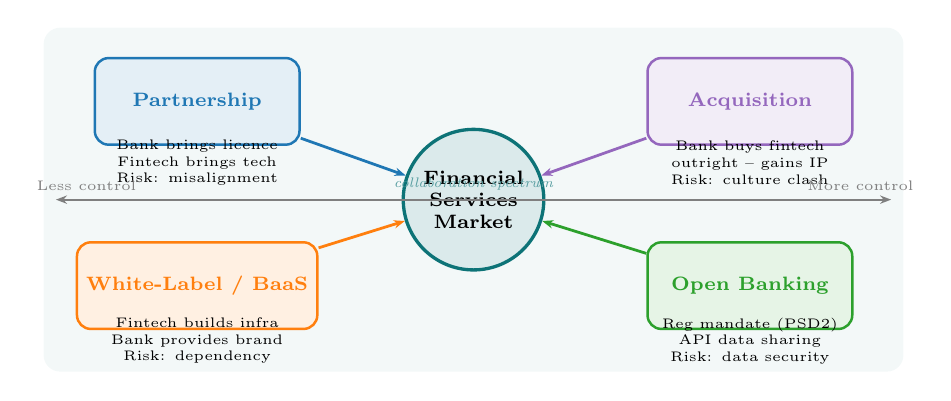
\begin{tikzpicture}[
    scale=0.78,
    box/.style={rectangle, rounded corners=5pt, minimum width=2.6cm,
                minimum height=1.1cm, align=center, font=\scriptsize\bfseries,
                line width=0.9pt},
    lbl/.style={font=\tiny, align=center, text width=2.4cm},
    arr/.style={-{Stealth[length=4pt]}, line width=1.0pt}
  ]

  % ---- Background ----
  \fill[mlteal!5, rounded corners=6pt] (-7.0,-2.8) rectangle (7.0,2.8);

  % ---- Central hub ----
  \node[circle, draw=mlteal, fill=mlteal!15, minimum size=1.5cm,
        font=\scriptsize\bfseries, align=center, line width=1.2pt]
    (hub) at (0,0) {Financial\\Services\\Market};

  % ---- Model 1: Partnership (top-left) ----
  \node[box, draw=mlblue, fill=mlblue!12] (part) at (-4.5,1.6)
    {\textcolor{mlblue}{Partnership}};
  \node[lbl] at (-4.5,0.6)
    {Bank brings licence\\Fintech brings tech\\Risk: misalignment};
  \draw[arr, mlblue] (part) -- (hub);

  % ---- Model 2: Acquisition (top-right) ----
  \node[box, draw=mlpurple, fill=mlpurple!12] (acq) at (4.5,1.6)
    {\textcolor{mlpurple}{Acquisition}};
  \node[lbl] at (4.5,0.6)
    {Bank buys fintech\\outright -- gains IP\\Risk: culture clash};
  \draw[arr, mlpurple] (acq) -- (hub);

  % ---- Model 3: White-Label / BaaS (bottom-left) ----
  \node[box, draw=mlorange, fill=mlorange!12] (wl) at (-4.5,-1.4)
    {\textcolor{mlorange}{White-Label / BaaS}};
  \node[lbl] at (-4.5,-2.3)
    {Fintech builds infra\\Bank provides brand\\Risk: dependency};
  \draw[arr, mlorange] (wl) -- (hub);

  % ---- Model 4: Open Banking (bottom-right) ----
  \node[box, draw=mlgreen, fill=mlgreen!12] (ob) at (4.5,-1.4)
    {\textcolor{mlgreen}{Open Banking}};
  \node[lbl] at (4.5,-2.3)
    {Reg mandate (PSD2)\\API data sharing\\Risk: data security};
  \draw[arr, mlgreen] (ob) -- (hub);

  % ---- Spectrum arrow ----
  \draw[{Stealth[length=4pt]}-{Stealth[length=4pt]}, mlgray, line width=0.8pt]
    (-6.8,0) -- (6.8,0);
  \node[font=\tiny, mlgray] at (-6.3,0.22) {Less control};
  \node[font=\tiny, mlgray] at (6.3,0.22) {More control};
  \node[font=\tiny\itshape, mlteal!70] at (0,0.25) {collaboration spectrum};

\end{tikzpicture}
\end{center}

\bottomnote{Slide 3/5 -- HOW | Most large banks employ \emph{all four} models simultaneously depending on the product and market.}
\end{frame}

% ===========================================================
%  SLIDE 4 of 5  --  WHERE
%  Visual: pgfplots grouped bar chart -- regional adoption
% ===========================================================
\begin{frame}{Where Is Fintech Winning? Global Adoption Patterns}

\vspace{-0.3em}
\begin{center}
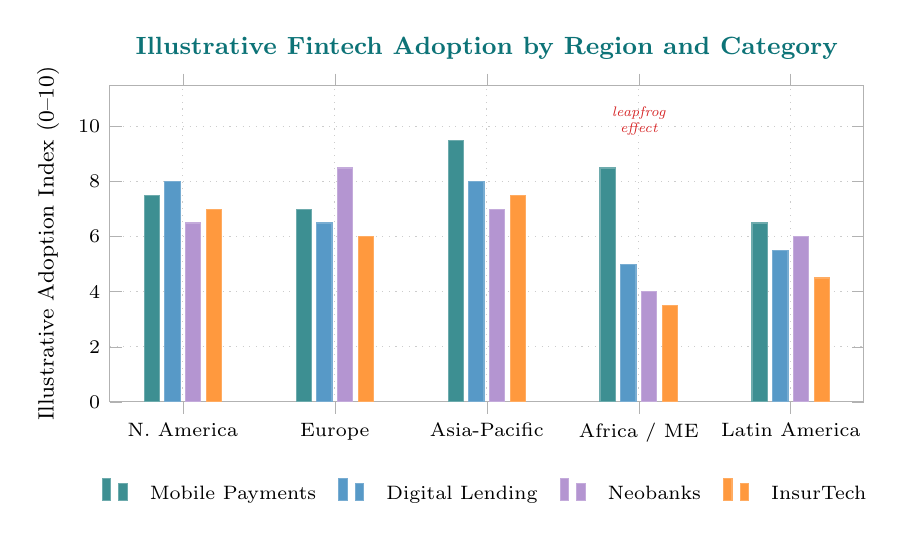
\begin{tikzpicture}
\begin{axis}[
    ybar,
    bar width=5.5pt,
    width=0.92\textwidth,
    height=5.6cm,
    enlarge x limits=0.12,
    ylabel={\footnotesize Illustrative Adoption Index (0--10)},
    ylabel style={font=\scriptsize},
    ymin=0, ymax=11.5,
    ytick={0,2,4,6,8,10},
    yticklabel style={font=\scriptsize},
    symbolic x coords={
      {N. America},
      {Europe},
      {Asia-Pacific},
      {Africa / ME},
      {Latin America}
    },
    xtick=data,
    xticklabel style={font=\scriptsize, align=center},
    legend style={
      at={(0.5,-0.22)},
      anchor=north,
      legend columns=4,
      font=\scriptsize,
      column sep=6pt,
      draw=none
    },
    legend cell align=left,
    grid=major,
    grid style={dotted, mlgray!40},
    axis line style={mlgray!60},
    tick style={mlgray!60},
    title={\small Illustrative Fintech Adoption by Region and Category},
    title style={font=\small\bfseries, color=mlteal}
  ]

  % Mobile Payments
  \addplot[fill=mlteal!80, draw=mlteal!60] coordinates {
    ({N. America},7.5) ({Europe},7.0) ({Asia-Pacific},9.5)
    ({Africa / ME},8.5) ({Latin America},6.5)
  };

  % Digital Lending
  \addplot[fill=mlblue!75, draw=mlblue!60] coordinates {
    ({N. America},8.0) ({Europe},6.5) ({Asia-Pacific},8.0)
    ({Africa / ME},5.0) ({Latin America},5.5)
  };

  % Neobanks
  \addplot[fill=mlpurple!70, draw=mlpurple!55] coordinates {
    ({N. America},6.5) ({Europe},8.5) ({Asia-Pacific},7.0)
    ({Africa / ME},4.0) ({Latin America},6.0)
  };

  % InsurTech
  \addplot[fill=mlorange!80, draw=mlorange!65] coordinates {
    ({N. America},7.0) ({Europe},6.0) ({Asia-Pacific},7.5)
    ({Africa / ME},3.5) ({Latin America},4.5)
  };

  \legend{Mobile Payments, Digital Lending, Neobanks, InsurTech}

  % Annotation: leapfrog
  \node[font=\tiny\itshape, text=mlred, align=center]
    at (axis cs:{Africa / ME}, 10.2)
    {leapfrog\\effect};

\end{axis}
\end{tikzpicture}
\end{center}
\vspace{-0.4em}
{\tiny\textcolor{mlgray}{\textit{Conceptual adoption levels -- illustrative comparison only. Actual metrics vary by source and definition.}}}

\bottomnote{Slide 4/5 -- WHERE | Regions with weaker traditional banking often leapfrog to mobile-first solutions (M-Pesa, Alipay, PIX).}
\end{frame}

% ===========================================================
%  SLIDE 5 of 5  --  SO WHAT
%  Visual: TikZ balance scale metaphor
% ===========================================================
\begin{frame}{So What? Innovation vs. Stability -- The Ongoing Balance}

\begin{center}
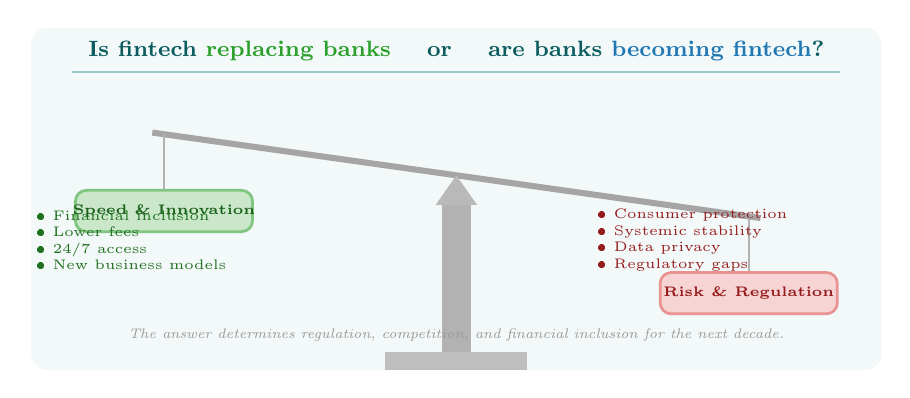
\begin{tikzpicture}[scale=0.75, every node/.style={font=\small}]

  % ---- Background ----
  \fill[mlteal!5, rounded corners=6pt] (-7.2,-2.8) rectangle (7.2,3.0);

  % ---- Scale base and pillar ----
  \fill[mlgray!60] (-0.25,-2.8) rectangle (0.25,0.0);  % pillar
  \fill[mlgray!50] (-1.2,-2.8) rectangle (1.2,-2.5);   % base

  % ---- Scale beam (tilted slightly left = innovation heavier) ----
  \def\tilt{8}  % degrees
  \draw[mlgray!70, line width=2.2pt]
    ({-5.2*cos(\tilt)},{0.5+5.2*sin(\tilt)}) --
    ({5.2*cos(\tilt)},{0.5-5.2*sin(\tilt)});

  % Fulcrum triangle
  \fill[mlgray!55]
    (-0.35,0.0) -- (0.35,0.0) -- (0.0,0.5) -- cycle;

  % ---- Left chain and pan (INNOVATION / INCLUSION -- heavier) ----
  \draw[mlgray!60, line width=0.9pt]
    ({-5.0*cos(\tilt)},{0.5+5.0*sin(\tilt)}) --
    ({-5.0*cos(\tilt)},{0.5+5.0*sin(\tilt)-1.3});

  \fill[mlgreen!25, draw=mlgreen!60, line width=1pt, rounded corners=4pt]
    ({-5.0*cos(\tilt)-1.5},{0.5+5.0*sin(\tilt)-1.3-0.35})
    rectangle
    ({-5.0*cos(\tilt)+1.5},{0.5+5.0*sin(\tilt)-1.3+0.35});

  % Items on left pan
  \pgfmathsetmacro{\lx}{-5.0*cos(\tilt)}
  \pgfmathsetmacro{\ly}{0.5+5.0*sin(\tilt)-1.3}
  \node[align=center, font=\tiny\bfseries, text=mlgreen!60!black] at (\lx,\ly)
    {Speed \& Innovation};

  % Left pan side labels (stacked coins/items)
  \node[font=\tiny, text=mlgreen!70!black, align=left]
    at (-5.5,-0.6)
    {\textbullet\ Financial inclusion\\
     \textbullet\ Lower fees\\
     \textbullet\ 24/7 access\\
     \textbullet\ New business models};

  % ---- Right chain and pan (RISK / REGULATION -- lighter) ----
  \draw[mlgray!60, line width=0.9pt]
    ({5.0*cos(\tilt)},{0.5-5.0*sin(\tilt)}) --
    ({5.0*cos(\tilt)},{0.5-5.0*sin(\tilt)-1.3});

  \fill[mlred!20, draw=mlred!50, line width=1pt, rounded corners=4pt]
    ({5.0*cos(\tilt)-1.5},{0.5-5.0*sin(\tilt)-1.3-0.35})
    rectangle
    ({5.0*cos(\tilt)+1.5},{0.5-5.0*sin(\tilt)-1.3+0.35});

  \pgfmathsetmacro{\rx}{5.0*cos(\tilt)}
  \pgfmathsetmacro{\ry}{0.5-5.0*sin(\tilt)-1.3}
  \node[align=center, font=\tiny\bfseries, text=mlred!70!black] at (\rx,\ry)
    {Risk \& Regulation};

  % Right pan side labels
  \node[font=\tiny, text=mlred!70!black, align=left]
    at (4.0,-0.6)
    {\textbullet\ Consumer protection\\
     \textbullet\ Systemic stability\\
     \textbullet\ Data privacy\\
     \textbullet\ Regulatory gaps};

  % ---- The core question ----
  \node[mlteal!80!black, font=\footnotesize\bfseries, align=center]
    at (0,2.6)
    {Is fintech \textcolor{mlgreen}{replacing banks} \quad or \quad
     are banks \textcolor{mlblue}{becoming fintech}?};

  \draw[mlteal!40, line width=0.5pt] (-6.5,2.25) -- (6.5,2.25);

  % ---- Bottom verdict ----
  \node[mlgray!80, font=\tiny\itshape, align=center] at (0,-2.2)
    {The answer determines regulation, competition, and financial inclusion for the next decade.};

\end{tikzpicture}
\end{center}

\bottomnote{Slide 5/5 -- SO WHAT | ``Fintech is not a technology story -- it is a governance story told in the language of technology.'' (L01 core thesis)}
\end{frame}

% ===========================================================
%  END
% ===========================================================
\end{document}
